%-*- coding: utf-8 -*-   
\documentclass[11pt,a4paper,a4wide,headsepline,bibtotoc,twoside]{scrbook}

\usepackage[T1]{fontenc}
\usepackage{ucs}
\usepackage[utf8x]{inputenc} 
\usepackage{lmodern}
%\usepackage{textcomp}
\usepackage{garamond}
\usepackage{helvet}
\usepackage{courier} % used to display code
\usepackage{color}
 \usepackage{anysize}
\marginsize{3cm}{2cm}{1cm}{1cm}
\textwidth 15 cm 

\definecolor{dkgreen}{rgb}{0,0.6,0}
\definecolor{gray}{rgb}{0.5,0.5,0.5}
\definecolor{mauve}{rgb}{0.58,0,0.82}

\definecolor{rltbrightred}{rgb}{1,0,0}
\definecolor{rltred}{rgb}{0.75,0,0}
\definecolor{rltdarkred}{rgb}{0.5,0,0}
%
\definecolor{rltbrightgreen}{rgb}{0,0.75,0}
\definecolor{rltgreen}{rgb}{0,0.5,0}
\definecolor{rltdarkgreen}{rgb}{0,0,0.25}
%
\definecolor{rltbrightblue}{rgb}{0,0,1}
\definecolor{rltblue}{rgb}{0,0,0.75}
\definecolor{rltdarkblue}{rgb}{0,0,0.5}

\definecolor{webred}{rgb}{0.5,.25,0}
\definecolor{webblue}{rgb}{0,0,0.75}
\definecolor{webgreen}{rgb}{0,0.5,0}
\definecolor{webbrightgreen}{rgb}{0,0.5,0}

\usepackage{listings}
\lstset{ %
  language=SQL,                % the language of the code
  basicstyle=\ttfamily,           % the size of the fonts that are used for the code
  numbers=left,                   % where to put the line-numbers
  numberstyle=\footnotesize,          % the size of the fonts that are used for the line-numbers
  stepnumber=2,                   % the step between two line-numbers. If it's 1, each line 
                                  % will be numbered
  numbersep=5pt,                  % how far the line-numbers are from the code
  backgroundcolor=\color{white},      % choose the background color. You must add \usepackage{color}
  showspaces=false,               % show spaces adding particular underscores
  showstringspaces=false,         % underline spaces within strings
  showtabs=false,                 % show tabs within strings adding particular underscores
  frame=single,                   % adds a frame around the code
  tabsize=2,                      % sets default tabsize to 2 spaces
  captionpos=b,                   % sets the caption-position to
                                % bottom 
  breaklines=true,                % sets automatic line breaking
  breakatwhitespace=false,        % sets if automatic breaks should only happen at whitespace
  title=\lstname,                   % show the filename of files included with \lstinputlisting;
                                  % also try caption instead of title
  numberstyle=\tiny\color{gray},        % line number style
  keywordstyle=\color{blue},          % keyword style
  columns=fixed,
  commentstyle=\color{dkgreen},       % comment style
  stringstyle=\color{mauve},         % string literal style
  escapeinside={\%*}{*)},            % if you want to add a comment within your code
  morekeywords={*,...}               % if you want to add more keywords to the set
} 
\usepackage[dvips]{thumbpdf}
\usepackage[pdftex,
colorlinks=true,
urlcolor=rltblue,               % \href{...}{...}
anchorcolor=rltbrightblue,
filecolor=rltgreen,             % \href*{...}
linkcolor=rltblue,               % \ref{...} and \pageref{...}
menucolor=webdarkblue,
citecolor=webbrightgreen,
pdftitle={Projecto de Fim de Curso},
pdfauthor={Pedro Moreira, 10015},
pdfsubject={Agrometeo Alentejo},
pdfkeywords={Estação meteorológica, agricultura, worpress},
% pdfadjustspacing=1,
pagebackref=false,
pdfpagemode=None,
bookmarksopen=true]{hyperref}
\pdfcompresslevel=9

\usepackage[pdftex]{graphicx}
\usepackage{thumbpdf}

%%%%%%%%%%%%%%%%%%%%%%%%%

%% escrita em portugues
%\usepackage[latin1]{inputenc}
\usepackage[portuges]{babel}

% virgulas numericas correctas
\usepackage{icomma}

% processamento com indicação de linhas pelo pacote xdvi
\usepackage{srcltx}

\bibliographystyle{plain}

%% introducao do ambiente de geracao de indices
\usepackage{makeidx}

\usepackage[isu,small,ruled]{caption}
\setlength{\captionmargin}{0.5cm}
\usepackage{prettyref}

%\usepackage[portuges]{minitoc}

%% pacotes matematicos AMS
\usepackage[intlimits]{amsmath}
\usepackage{amssymb}

% simbolos matematicos
%\usepackage{jeffe}
%% graficos com dvips
%%
%%
%%
%% as fontes para os graficos são de 12pt, helvetica
% \usepackage[dvips]{graphics}
\usepackage{lscape}
\usepackage{subfigure}

% captions
\usepackage{float}
\usepackage{rotating}

%% bibliografia por temas e capitulos
%\usepackage{bibtopic}

%% especificacoes para portugues
\newrefformat{teorema}{Teorema~\ref{#1}}
\newrefformat{cha}{Cap{\'\i}tulo~\ref{#1}}
\newrefformat{sec}{Sec{\c c}{\~a}o~\ref{#1}}
\newrefformat{tab}{Tab.~\ref{#1}}
\newrefformat{eq}{Eq.~\ref{#1}}
\newrefformat{def}{Def.~\ref{#1}}
%% na p{\'a}g. #2}
\newrefformat{fig}{Fig.~\ref{#1}}
%% na p{\'a}g. #2}
\newrefformat{alg}{Alg.~\ref{#1}}
%%\newrefformat{pag}{P{\'a}g.~\ref{#1}}

\newtheorem{assuncao}{Assun{\c c}{\~a}o}
\newtheorem{definicao}{Defini{\c c}{\~a}o}
\newtheorem{teorema}{Teorema}

\newcommand{\goodgap}{%
\hspace{\subfigtopskip}%
\hspace{\subfigbottomskip}}

\newcommand\glossaryname{Gloss{\'a}rio}

% processamento mais agradável de figuras
\renewcommand{\topfraction}{0.85}
\renewcommand{\textfraction}{0.1}
\renewcommand{\floatpagefraction}{0.75}

%%% fontes para cabecalhos e inicios de capitulos
%%% \renewcommand{\sectfont}{\rmfamily\bfseries}

%\renewcommand{\headfont}{\scshape}


%%% novas declaracoes para amsmath.sty
%\DeclareMathOperator{\argmax}{argmax}
\def\argmax{\operatornamewithlimits{arg\,max}}
\DeclareMathOperator{\tgh}{tgh}
\DeclareMathOperator{\arctg}{arctg}
\DeclareMathOperator{\arcsen}{arcsen}
\DeclareMathOperator{\sen}{sen}
\DeclareMathOperator{\erf}{erf}
\DeclareMathOperator{\ud}{d}
\DeclareMathOperator{\jacobian}{J}
\DeclareMathOperator{\abs}{abs}
\DeclareMathOperator{\cov}{cov}
\DeclareMathOperator{\signum}{sgn}
\DeclareMathOperator{\decibel}{dB}
\DeclareMathOperator{\pixel}{pixel}
\DeclareMathOperator{\verdade}{\mathbf{Verdade}}
\DeclareMathOperator{\falso}{\mathbf{Falso}}
\DeclareMathOperator{\probcdf}{Pr}


%%
\usepackage{supertabular}

% posicionamento arbitrario de texto
\usepackage[absolute]{textpos}
\usepackage{type1cm}
\usepackage{lettrine}
\usepackage{multind}
\makeindex{aut}
\makeindex{alf}

\begin{document}

\garamond
%% modos de armazenamento de imagens em Postscript encapsulado
%% e comprimido
\DeclareGraphicsRule{eps.gz}{eps}{eps.bb}{`gunzip -c #1}
%% directoria onde se armazena os ficheiros
\graphicspath{{EPS/}}

%% \symbol{64} corresponde a @
%% parte frontal da tese
\frontmatter
%\maketitle
\thispagestyle{empty}
\begin{titlepage}
  \vspace*{2cm}
  \baselineskip=24pt

\fontshape{bold}
\fontsize{20}{30}
  \textblockorigin{0cm}{0cm}
  \begin{textblock*}{16cm}(2.5cm,2.5cm)
    \centering
    \textbf{{INSTITUTO POLITÉCNICO DE BEJA
  \end{textblock*}

   \textblockorigin{0cm}{3cm}
   \begin{textblock*}{16cm}(2.5cm,3cm)
     \centering
\fontshape{bold}	
\fontsize{24}{30}
       \textbf{{Projecto de Fim de Curso
\end{textblock*}




   \textblockorigin{0cm}{3cm}
	\centering
   \begin{textblock*}{15cm}(3cm,8cm)
     \centering
      
 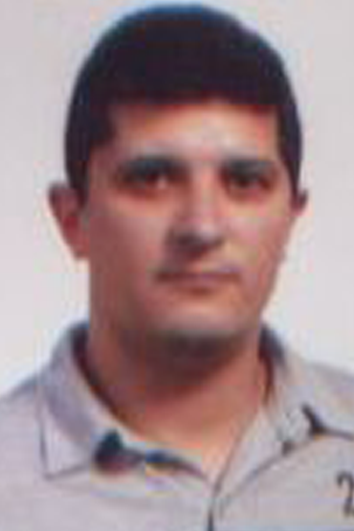
\includegraphics[width=3cm]{pedro.png}
	
   \end{textblock*}


   \textblockorigin{0cm}{5cm}
   \begin{textblock*}{16cm}(2.5cm,13cm)
     \centering
\fontshape{bold}	
\fontsize{16}{16}
       \textbf{{Pedro Miguel Clemente Dias Moreira\\}}
   \end{textblock*}
   \textblockorigin{0cm}{5cm}
   \begin{textblock*}{16cm}(2.5cm,14cm)
     \centering
\fontshape{bold}	
\fontsize{16}{16}
       \textbf{{n.º 10015\\}}
   \end{textblock*}


   \textblockorigin{0cm}{5cm}
   \begin{textblock*}{16cm}(2.5cm,21.2cm)
     \centering
\fontshape{bold}	
\fontsize{12}{20}
       \textbf{17 de março 2012}
   \end{textblock*}
   
\end{titlepage}
%%
%% capa.tex
%% 
%% Made by Pedro Moreira
%% Email   <mail@pedromoreira.org>
%% 
%% Started on  Sun Jun 17 01:17:00 2012 Pedro Moreira
%% Last update Sun Jun 17 23:50:33 2012 Pedro Moreira
%%

\thispagestyle{empty}
\cleardoublepage


%% corpo do livro
\mainmatter
%% realizacao de miniindices de conteudo


\cleardoublepage
\pagestyle{headings}
\setcounter{page}{1}
\pagenumbering{arabic}
%\addcontentsline{toc}{section}{Contents}
\addcontentsline{toc}{section}{Índice Geral}
\tableofcontents
\cleardoublepage
% \addcontentsline{toc}{section}{Lista de Figuras}
 %\listoffigures
 %\cleardoublepage
% \addcontentsline{toc}{section}{Lista de Tabelas}
 %\listoftables
 %\cleardoublepage
%% \include{listasimbolos}
%\cleardoublepage
%\pagestyle{headings}
%\setcounter{page}{1}
%\pagenumbering{arabic}

%%\part{}

\chapter{Resumo}
\label{chap:intro}
Este trabalho abrange a criação de uma rede de estações meteorológicas no Baixo Alentejo. O mesmo apresenta um estudo sobre projectos semelhantes a nível mundial, quais as vantagens e problemas existentes nas implementações apresentadas.
O trabalho pode ser dividido em três grandes áreas:
\subsection*{Recolha de dados}
\label{sec:recolha_dados}
Nesta secção são apresentados projectos semelhantes, a forma como recolhem os d secção ados, o tipo de equipamentos utilizados no processo, as principais vantagens e dificuldades de um sistema do mesmo tipo.
\subsection*{Envio dos dados para o instituto de meteorologia e obtenção de previsões meteorológicas}
O documento apresenta a forma como é armazenada a informação e, posteriormente, enviada para o Instituto de Meteorologia para a obtenção das previsões meteorológicas para cada um dos locais onde se encontra uma estação meteorológica.
\subsection*{Interface}
Nesta secção é apresentado um estudo sobre os tipos de interfaces existentes para consulta de previsoes meteorológicas, bem como a explicação da criação de um interface para o sistema em causa.

\cleardoublepage
\chapter{Recolha de Dados}
\label{chap:recolha_dados}
Após uma pesquisa sobre sistemas semelhantes foram encontrados três considerados úteis para o estudo em causa, dois estarngeiros e um nacional. O Nacional

\cleardoublepage
\bibliography{bibliografia}


\end{document}
